\section{Lenti}
Tutte le lenti obbediscono alla legge di snell sulla rifrazione, di conseguenza la geometria della lente determina come la luce si propaga attraverso gli elementi ottici, stabiliremo ora un glossario con la terminologia e introdurremo diverse geometrie di lenti.

\subsection{Terminologia}

\begin{tabularx}{\textwidth}{l p{.8\textwidth}}

D               & 	Diametro – Dimensione fisica della lente.\\
R               &	Raggio di curvatura – La distanza diretta tra il vertice di una superfice e il centro di curvatura.\\
EFL 	        &   Lunghezza focale effettiva – Distanza ottica tra il piano principale di un ottica e il piano immagine.\\
BFL 	        &   Lunghezza focale posteriore – Distanza meccanica tra l'ultima superficie della lente ed il piano immagine.\\
P, P" 	        &   Piano Principale – Piano ipotetico dove i raggi di luce incidenti si piegano a causa del fenomeno della rifrazione.\\
CT              & 	Spessore centrale – la distanza tra il piano principale e la fine dell'elemento.\\
db 	            &   Diametro di ingresso del raggio – Diametro di un raggio collimato in ingresso.\\
dr 	            &   Exit Beam Diameter – Diametro di un anello luminoso in uscita all'elemento.\\
L 	            &   Lunghezza distanza effettiva fra le superfici di un elemento.
\end{tabularx}

\subsection{Plano Convex}

Ideal for collimation and focusing applications utilizing monochromatic
illumination. Note: Orient the curved surface of a PCX lens towards the source
for optimal performance.

\begin{figure}[!ht]
\centering

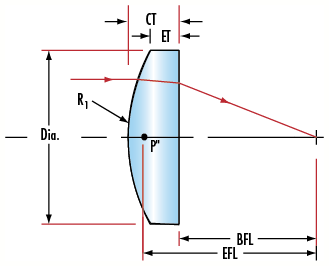
\includegraphics[width=.3\textwidth]{img/plano-convex.png}

\caption{Lente Plano-Convex}
\label{fig:ccd-blockdiagram}
\end{figure}


\subsection{Double Convex}

Ideal for image relay, and for imaging of objects at close conjugates. Note:
Aberrations will increase as the conjugate ratios increase.

\begin{figure}[!ht]
\centering

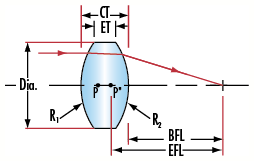
\includegraphics[width=.3\textwidth]{img/double-convex.png}

\caption{Lente Plano-Convex}
\label{fig:ccd-blockdiagram}
\end{figure}

\subsection{Plano Concave}
Comprised of one flat and one inward curved surface. Ideal for beam expansion, light projection, and expanding the focal length of an optical system. 

\begin{figure}[!ht]
\centering

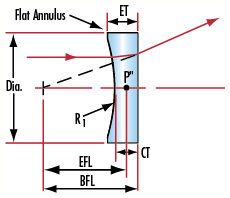
\includegraphics[width=.3\textwidth]{img/plano-concave.png}

\caption{Lente Plano-Convex}
\label{fig:ccd-blockdiagram}
\end{figure}


\subsection{Double Concave}
Comprised of two inward, equally curved surfaces. Ideal for beam expansion, light projection, and expanding the focal length of an optical system. 
\begin{figure}[!ht]
\centering

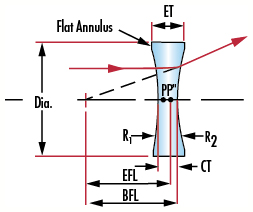
\includegraphics[width=.3\textwidth]{img/double-concave.png}

\caption{Lente Plano-Convex}
\label{fig:ccd-blockdiagram}
\end{figure}

\subsection{Acromatica positiva}
Performs similar function as a PCX or DCX lens, but can provide smaller spot sizes and superior image quality. Achromatic lenses are useful for reducing spherical and chromatic aberration
\begin{figure}[!ht]
\centering

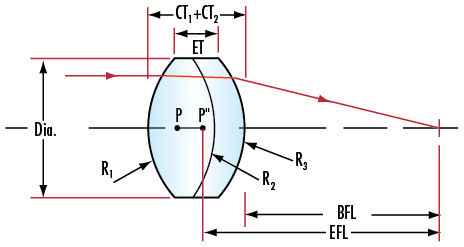
\includegraphics[width=.3\textwidth]{img/positiva-acromatica.png}

\caption{Lente Plano-Convex}
\label{fig:ccd-blockdiagram}
\end{figure}

\subsection{Asferica}
Ideal for laser focusing or for replacing multiple spherical lens elements in a system. Useful for eliminating spherical aberration and greatly reducing other aberrations.

\begin{figure}[!ht]
\centering

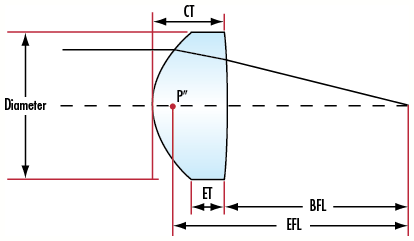
\includegraphics[width=.3\textwidth]{img/asferica.png}

\caption{Lente Plano-Convex}
\label{fig:ccd-blockdiagram}
\end{figure}



